%%%%%%%%%%%%%%%%%%%%%%%%%%%%%%%%%%%%%%%%%
% Jacobs Landscape Poster
% LaTeX Template
% Version 1.0 (29/03/13)
%
% Created by:
% Computational Physics and Biophysics Group, Jacobs University
% https://teamwork.jacobs-university.de:8443/confluence/display/CoPandBiG/LaTeX+Poster
% 
% Further modified by:
% Nathaniel Johnston (nathaniel@njohnston.ca)
%
% This template has been downloaded from:
% http://www.LaTeXTemplates.com
%
% License:
% CC BY-NC-SA 3.0 (http://creativecommons.org/licenses/by-nc-sa/3.0/)
%
%%%%%%%%%%%%%%%%%%%%%%%%%%%%%%%%%%%%%%%%%

%----------------------------------------------------------------------------------------
%	PACKAGES AND OTHER DOCUMENT CONFIGURATIONS
%----------------------------------------------------------------------------------------

\documentclass[final]{beamer}

\usepackage[scale=1.13]{beamerposter} % Use the beamerposter package for laying out the poster

\usetheme{confposter} % Use the confposter theme supplied with this template

\setbeamercolor{block title}{fg=Cerulean,bg=white} % Colors of the block titles
\setbeamercolor{block body}{fg=black,bg=white} % Colors of the body of blocks
\setbeamercolor{block alerted title}{fg=white,bg=Cerulean!100} % Colors of the highlighted block titles
\setbeamercolor{block alerted body}{fg=black,bg=Cerulean!20} % Colors of the body of highlighted blocks
% Many more colors are available for use in beamerthemeconfposter.sty

%-----------------------------------------------------------
% Define the column widths and overall poster size
% To set effective sepwid, onecolwid and twocolwid values, first choose how many columns you want and how much separation you want between columns
% In this template, the separation width chosen is 0.024 of the paper width and a 4-column layout
% onecolwid should therefore be (1-(# of columns+1)*sepwid)/# of columns e.g. (1-(4+1)*0.024)/4 = 0.22
% Set twocolwid to be (2*onecolwid)+sepwid = 0.464
% Set threecolwid to be (3*onecolwid)+2*sepwid = 0.708

\newlength{\sepwid}
\newlength{\onecolwid}
\newlength{\twocolwid}
\newlength{\threecolwid}
\setlength{\paperwidth}{48in} % A0 width: 46.8in
\setlength{\paperheight}{48in} % A0 height: 33.1in
\setlength{\sepwid}{0.018\paperwidth} % Separation width (white space) between columns
\setlength{\onecolwid}{0.27\paperwidth} % Width of one column
\setlength{\twocolwid}{0.33\paperwidth} % Width of two columns
\setlength{\threecolwid}{0.27\paperwidth} % Width of three columns
\setlength{\topmargin}{-0.5in} % Reduce the top margin size
%-----------------------------------------------------------

\usepackage{graphicx}  % Required for including images
\usepackage{tikz} % for header bar images
\usepackage{booktabs} % Top and bottom rules for tables
\usepackage{hyperref}
\usepackage{fixltx2e}
\usepackage[none]{hyphenat} % Get rid of hyphens

%----------------------------------------------------------------------------------------
%	TITLE SECTION 
%----------------------------------------------------------------------------------------

\title{Pedigree-based approaches to identifying selection in modern maize} % Poster title

\author{Kate Crosby$^{1}$, Oscar "Howie" Smith$^{1}$, \& Jeffrey Ross-Ibarra$^{1,2,3}$} % Author(s)

\institute{$^{1}$UC Davis, Department of Plant Sciences, $^{2}$UC Davis, Center For Population Biology, $^{3}$UC Davis, Genome Center} % Institution(s)

%----------------------------------------------------------------------------------------

\begin{document}

\addtobeamertemplate{headline}{} 
{
\begin{tikzpicture}[remember picture,overlay] 
\node [shift={(-12 cm,-8cm)}] at (current page.north east) {
\includegraphics[height=4.5cm]{download.jpeg}}; 
\end{tikzpicture} 
}
\addtobeamertemplate{headline}{} 
{
\begin{tikzpicture}[remember picture,overlay] 
\node [shift={(-3 cm,-8cm)}] at (current page.north east) {
\includegraphics[height=4.55cm]{rilab_logo.jpeg}}; 
\end{tikzpicture} 
}


\addtobeamertemplate{block end}{}{\vspace*{2ex}} % White space under blocks
\addtobeamertemplate{block alerted end}{}{\vspace*{2ex}} % White space under highlighted (alert) blocks

\setlength{\belowcaptionskip}{2ex} % White space under figures
\setlength\belowdisplayshortskip{2ex} % White space under equations

\begin{frame}[t] % The whole poster is enclosed in one beamer frame

\begin{columns}[t] % The whole poster consists of three major columns, the second of which is split into two columns twice - the [t] option aligns each column's content to the top

\begin{column}{\sepwid}\end{column} % Empty spacer column

\begin{column}{\onecolwid} % The first column

%----------------------------------------------------------------------------------------
%	ABSTRACT
%----------------------------------------------------------------------------------------

\begin{alertblock}{Abstract}
Modern maize has resulted from generations of mass selection for fitness (yield, standability, maturity, pest resistance, etc). Yet, in terms of adaptation, data from genome scans have largely fallen short in identifying the molecular signals of selection in modern maize. This shortcoming may be due to the failure to account for population structure in the data. Here we explore whether inclusion of pedigree data allows for the identification of weak selection and selection on standing variation. We used reduced-representation genotype-by-sequence (GBS) data from more than 2000 maize inbred lines representing over 60 years of the worldwide maize germplasm. We initially reconstructed pedigree graphs with historical information alone, and then pruned them using identity-by-state (IBS) information. We intend to evaluate the power of our pedigree approach to identify loci targeted by selection during modern maize breeding. These loci will then be associated with phenotypic traits using novel population/quantitative genomics approaches.
\end{alertblock}

%----------------------------------------------------------------------------------------
%	INTRODUCTION
%----------------------------------------------------------------------------------------

\begin{block}{Introduction}
Modern maize inbreds have undergone repeated rounds of natural selection through time. Yield has increased through the years, and other traits such as leaf angle show dramatic directional change as well. Yet few signals of molecular selection have been found across and/or within heterotic groups, possibly due to the failure to account for population structure \cite{Gerke:2013tw}. Pedigrees, built using a combination of historical parentage information and genetic data, can account for very minute population structure. While many pedigree records of historical parentage are incomplete or do not yet have affiliated genotypic data, there is still overlap between classic inbred accessions with parentage information that had GBS information. 

\end{block}


%------------------------------------------------
\begin{block}{Approaches}


We collected over 2000 historical parentage records for US modern maize from: 
\begin{enumerate}
\item Inbreds from USDA GRIN 
\item Gerdes and Tracy \cite{gerdes1993compilation}
\item Input from breeders and experts
\end{enumerate}

\par
This information was then paired with reduced representation sequence data from GBS 2.7 \cite{Glaubitz:2014eu} aligned to B73 ref. genome version 3, and a concordant dataset was produced.
\par

\begin{enumerate}
\item Pedigree graphs were constructed from historic data alone.
\item Pairwise kinship similarity was evaluated using Tassel \cite{Bradbury:2007fd} for known close relationships 
\item Pedigree relationships were then weighted by kinship similarity, and edges pruned based on similarity values
\item Finally, the segregation of alleles from heterozygous parents were tracked to offspring.
\end{enumerate}


\end{block}

\begin{alertblock}{Weighting pedigree graph}
The occasional lack of concordance between the pedigree and the values produced from the kinship similarity matrix in Tassel meant that there were most likely errors in the pedigree records. To reconstruct the pedigree "graph" (G) we weighted "edges" (E) (connections between vertices (V)) by the kinship values in the similarity matrix :
\par
\par
$$G = (w_{ij} * E_{ij}, V)$$
\par
\par
For inbred parent to children kinship similarity values below 1.0 were discarded.

\end{alertblock}

%----------------------------------------------------------------------------------------

\end{column} % End of the first column

\begin{column}{\sepwid}\end{column} % Empty spacer column

\begin{column}{\onecolwid} % The second column

%----------------------------------------------------------------------------------------
%	Overall pedigree
%----------------------------------------------------------------------------------------
\begin{block}{Pedigree graphs from historical records}
We first used historical records to construct a series of directed, unweighted maize pedigree graphs (Figure 1).  
\begin{figure}

\includegraphics[width=1.0\linewidth]{pedigree_poster.pdf}
\caption{A portion of the modern maize pedigree with a focus on B73 (PI 550473). Length of connections do not indicate relatedness, nor does size of node indicate importance.} 
\end{figure}

\end{block}

%----------------------------------------------------------------------------------------
%	Kinship
%----------------------------------------------------------------------------------------

\begin{block}{Kinship similarity as edge penalty}
Subsets of this larger pedigree were used to examine directed parent-child relationships as well as full-sibling and half-sibling relationships. An example is shown below with B73 and its direct children. As some of these pedigrees were incomplete, cut-off values from kinship similarity matrices were used to validate historical records of relatives (parent-child and siblings) (Figure 2). 
\begin{figure}
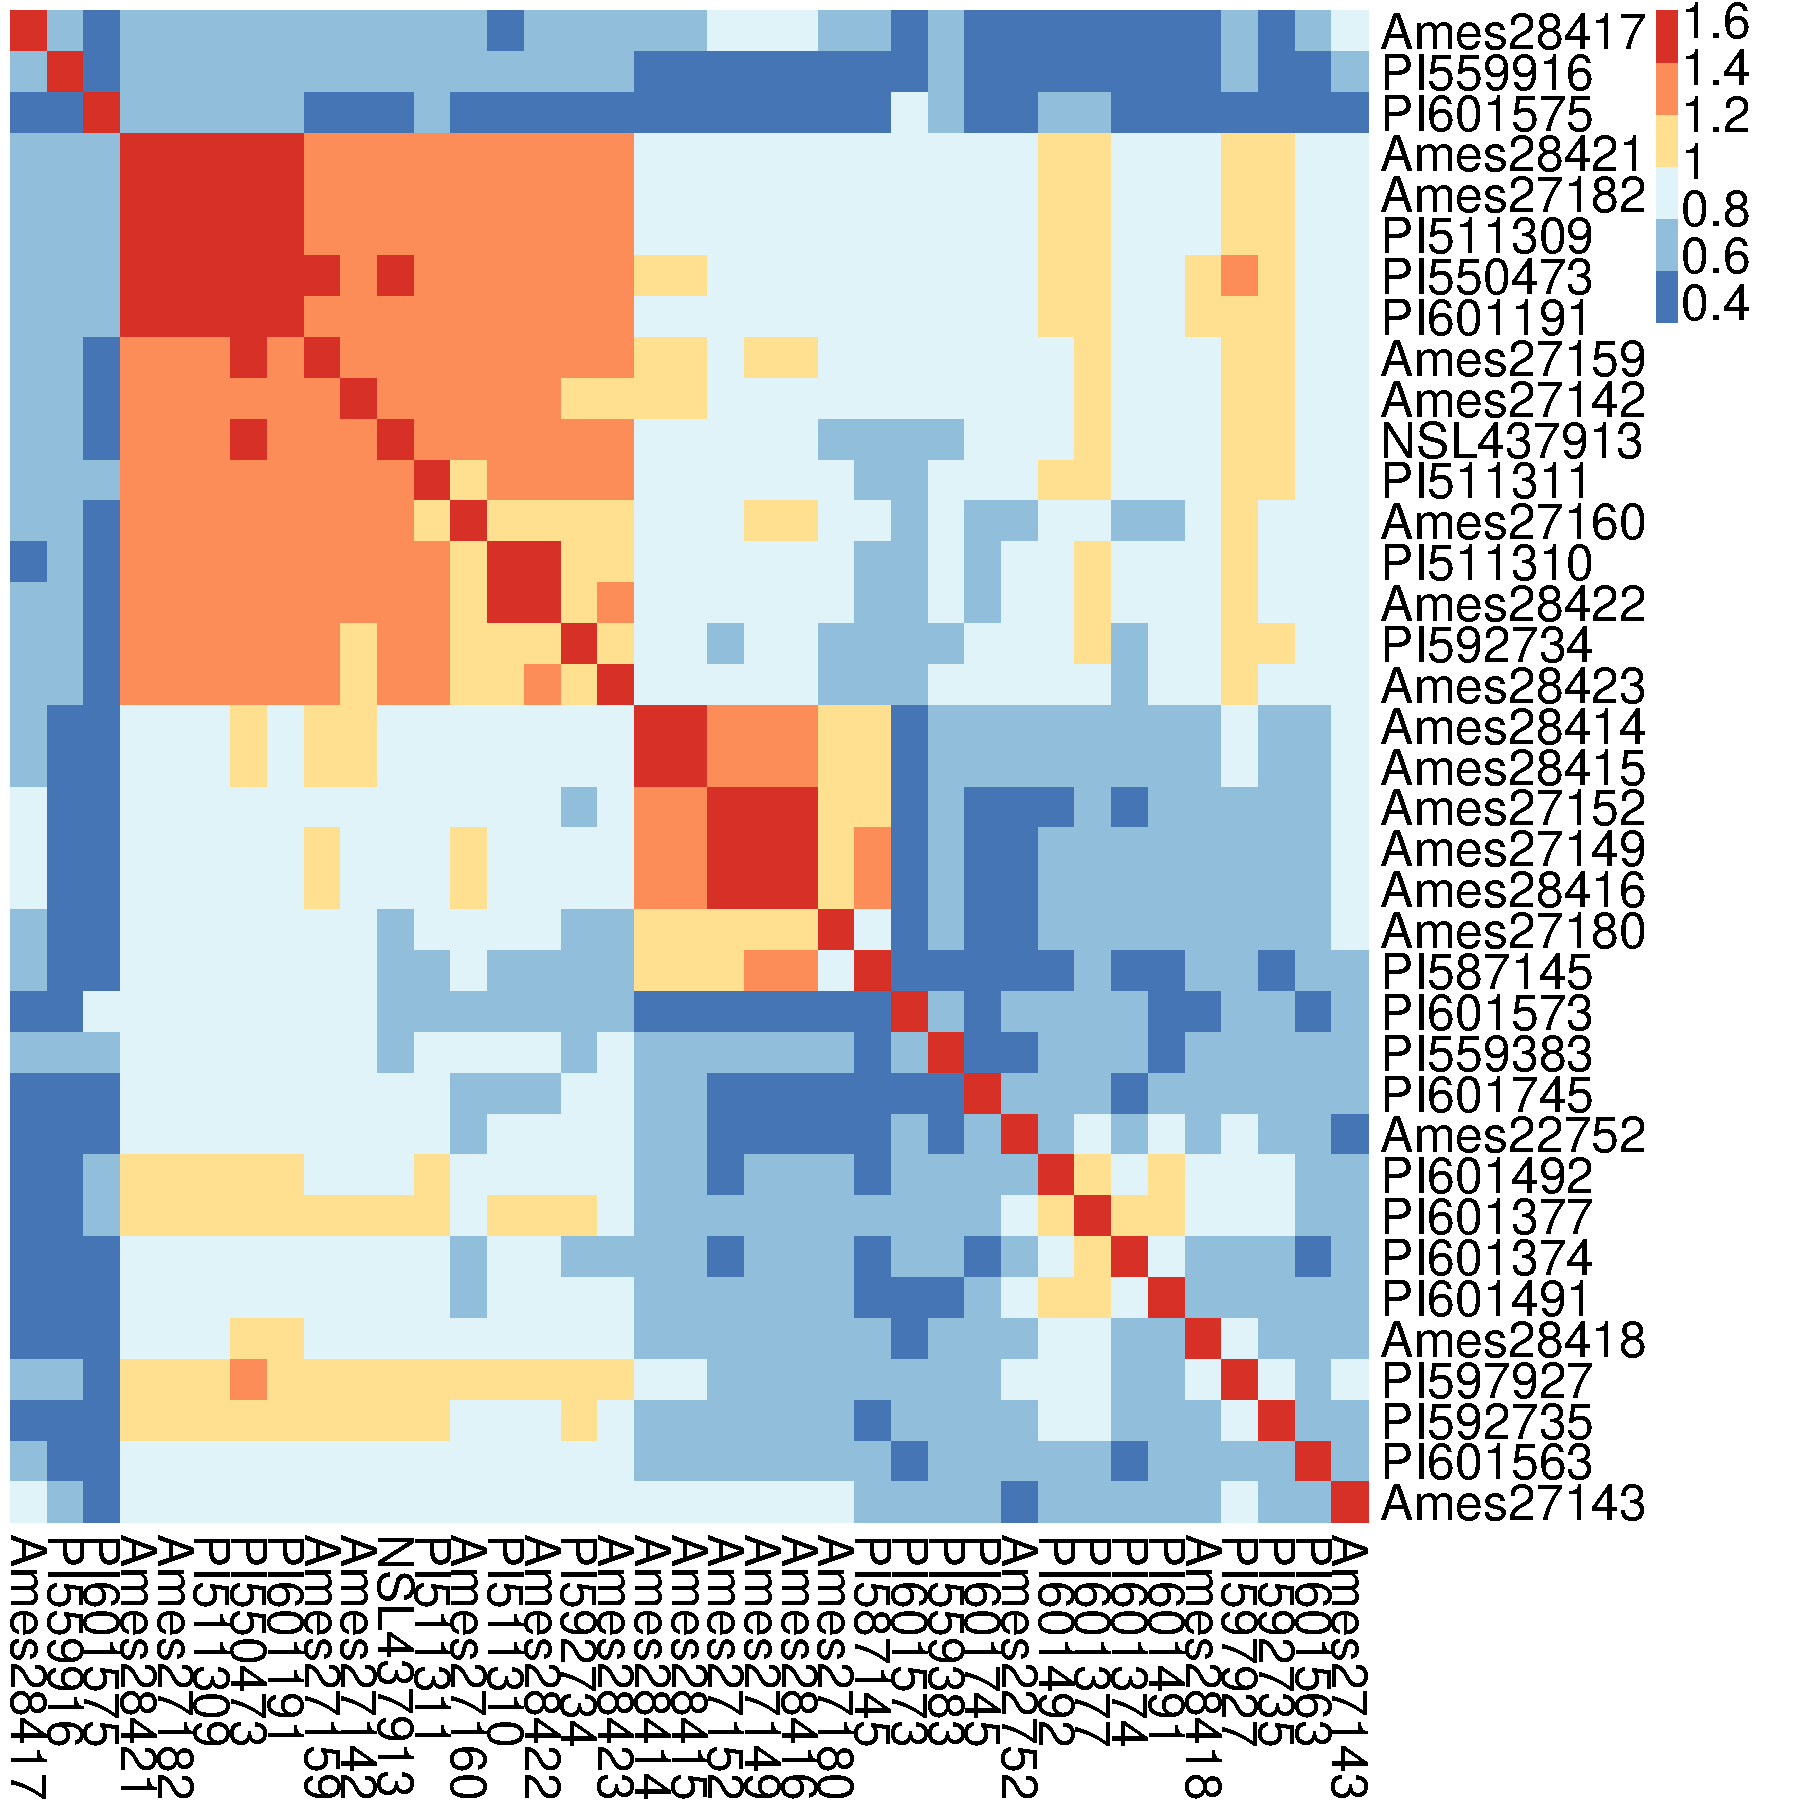
\includegraphics[width=1.0\linewidth]{Rplot02.pdf}
\caption{The pairwise kinship similarity matrix of B73 (PI 550473), and all its children from GBS 2.7 data}.
\end{figure}
\end{block}
%----------------------------------------------------------------------------------------

%----------------------------------------------------------------------------------------
%	REFERENCES
%----------------------------------------------------------------------------------------

\begin{block}{References}

\nocite{*} % Insert publications even if they are not cited in the poster
\small{\bibliographystyle{unsrt}
\bibliography{sample}\vspace{0.08in}}

\end{block}

\end{column} % End of the second column

\begin{column}{\sepwid}\end{column} % Empty spacer column

\begin{column}{\onecolwid} % The third column

%----------------------------------------------------------------------------------------
%	PEDIGREES ILLUSTRATED
%----------------------------------------------------------------------------------------
\begin{block}{Weighted pedigree}
The pedigree of B73 with edges to children now weighted by kinship similarity (Figure 3).
\begin{figure}
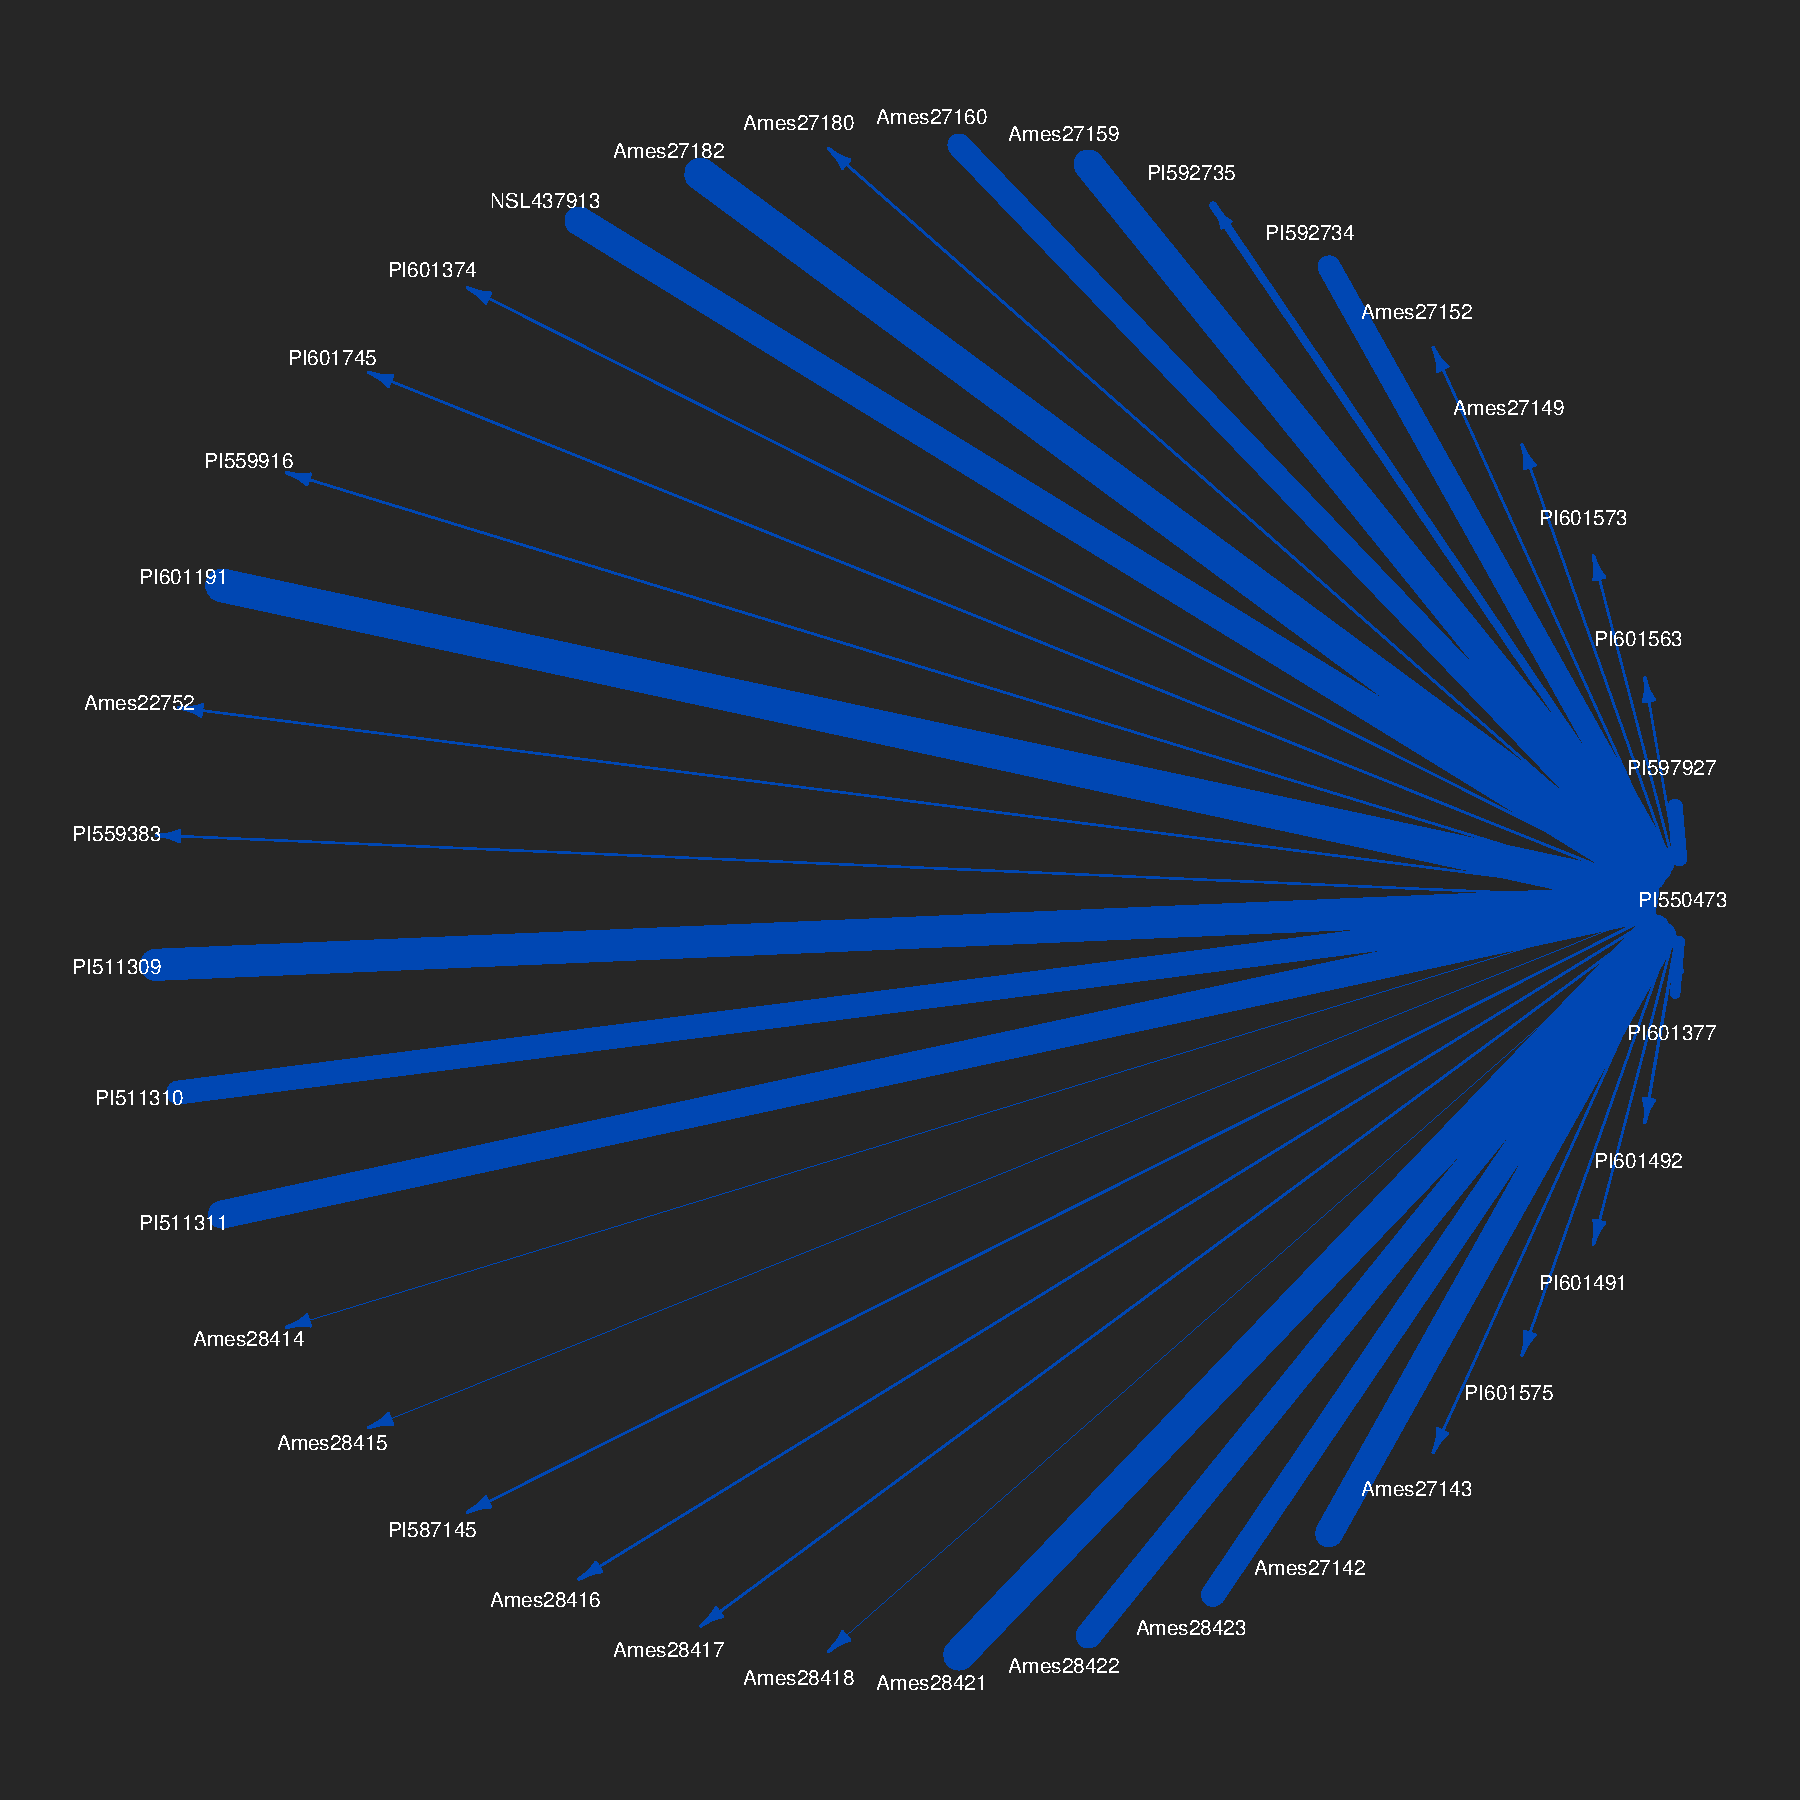
\includegraphics[width=1.0\linewidth]{weighted.pdf}
\caption{Weighted pedigree graph, where edge width indicates degree of similarity. Values of similarity below 1.0 were pruned - see BOX 1}.
\end{figure}

\end{block}


\begin{block}{Pruned pedigree}
Once the pedigree is pruned, heterozygous loci in B73 (or any other parent of interest) may then be evaluated for distorted segregation in its children (Figure \ref{fig:het_seg}).For example, B73 is heterozygous at 379 sites (indels not included). If one allele is disproportionately represented in the next generation (Figure \ref{fig:het_seg}) then this may indicate directional selection at a locus either within a small pedigree or across the entire pedigree.
\begin{figure}
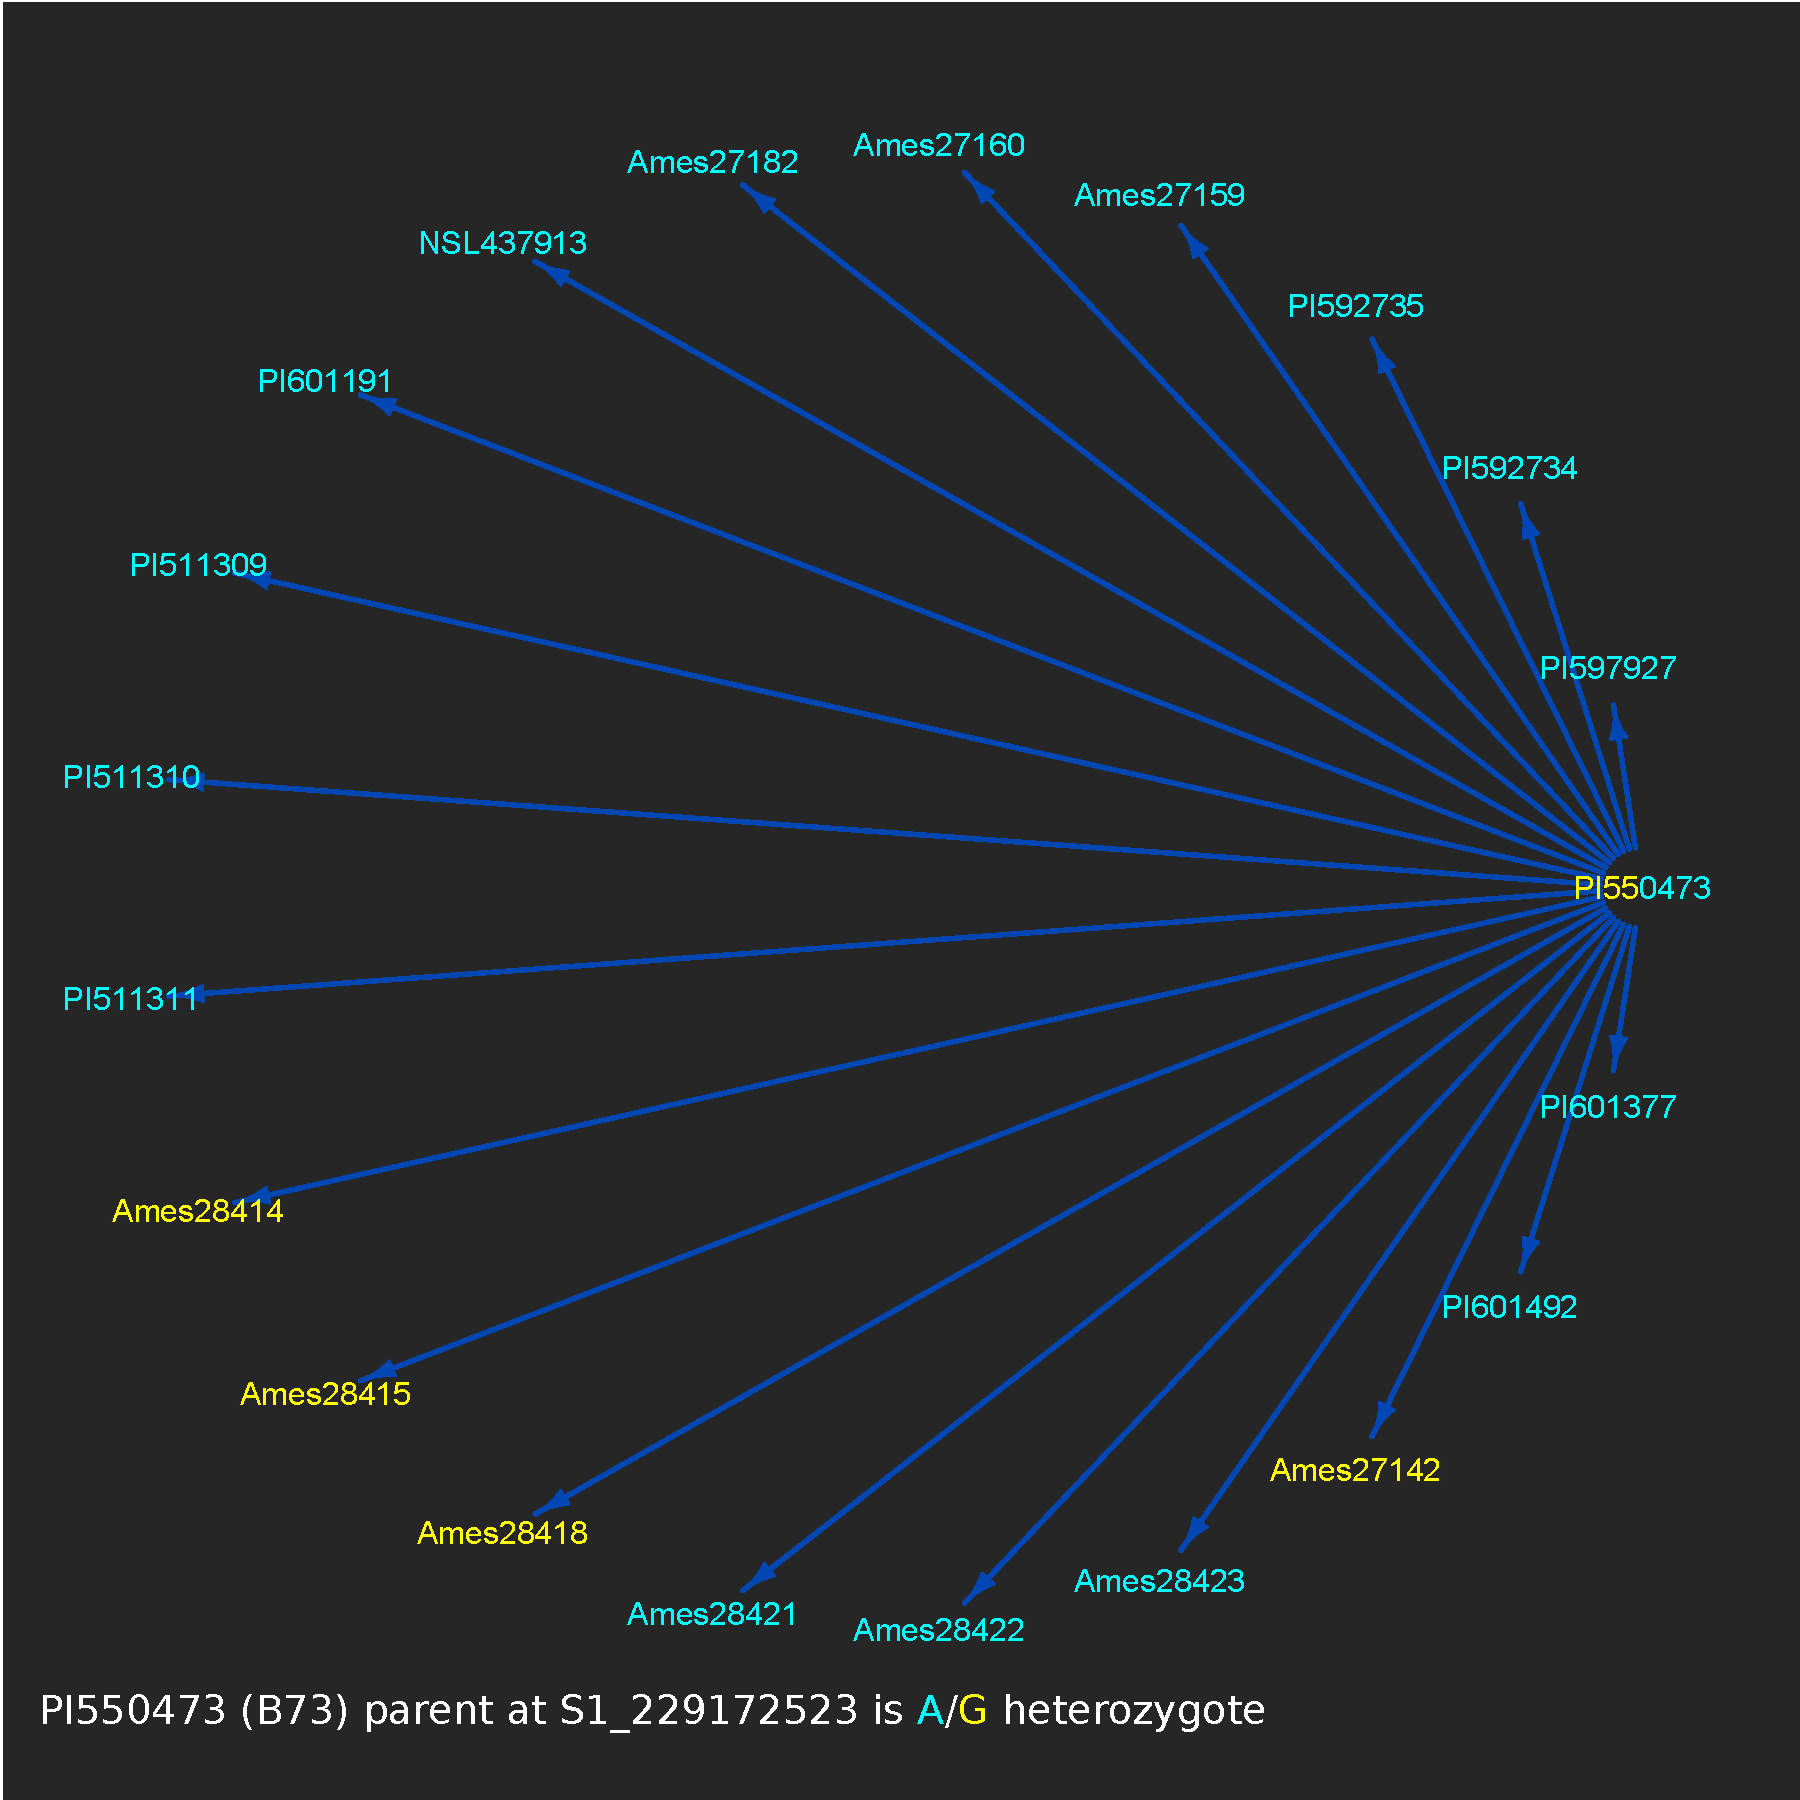
\includegraphics[width=1.0\linewidth]{Pruned.pdf}
\caption{Pruned pedigree graph, exemplifying segregation of alleles at a heterozygous locus in B73 parent}.
\label{fig:het_seg}%half the fun of figures in Latex is the label and using /ref!!
\end{figure}

\end{block}

\setbeamercolor{block title}{fg=Cerulean,bg=white} % Change the block title color

%----------------------------------------------------------------------------------------
%	ACKNOWLEDGEMENTS
%----------------------------------------------------------------------------------------

\begin{block}{Acknowledgements}

\small{\rmfamily{We thank Dupont Pioneer and the USDA for funding this project. We also thank Justin Gerke for invaluable input and expertise.}} \\

\end{block}




%----------------------------------------------------------------------------------------

\end{column} % End of the third column

\end{columns} % End of all the columns in the poster

\end{frame} % End of the enclosing frame

\end{document}
